\section*{Introduction}
\addcontentsline{toc}{section}{Introduction}
\dots
\newpage
\section{Résumé}

\section{Cadrage}
\subsection{Finalités et importance du projet}
L’analyse tactique dans les sports collectifs connaît une croissance exponentielle grâce aux avancées en vision par ordinateur et en apprentissage automatique (\emph{Machine Learning}). Ces technologies permettent aujourd’hui de comprendre et d’optimiser les stratégies de jeu avec une précision et une profondeur sans précédent.

Le projet \textbf{TactIAque} s’inspire des récents travaux de \textbf{RoboFlow}, une initiative pionnière visant à améliorer les algorithmes d’analyse tactique pour le football. Toutefois, le basketball reste un domaine encore sous-exploré dans ce contexte, offrant une opportunité unique de développement et d’innovation. Ce projet se concentre donc sur le basketball, avec pour objectif de fournir des outils robustes pour l’analyse des tactiques dans ce sport collectif.

En combinant des méthodologies existantes et des innovations spécifiques au basketball, \textbf{TactIAque} vise à combler cette lacune en proposant des solutions adaptées aux exigences de ce sport.
\paragraph{Hypothèses de lancement}
    \subparagraph{Compétences des membres de l'équipe}
    \subparagraph{Moyens techniques à disposition}
    \subparagraph{Obstacles à lever}
    \subparagraph{Analyse SWOT}
    L’analyse SWOT met en évidence les éléments clés influençant la réussite du projet. Voir la figure \ref{tab:swot}
    \begin{table} [!h]
        \centering  
        \begin{tabular}{|p{7cm}|p{7cm}|}  
        \hline  
        \textbf{Forces (Strengths)} & \textbf{Faiblesses (Weaknesses)} \\  
        \hline  
        \begin{itemize}
        \item Disponibilité de modèles performants comme RT-DETR, reconnus pour leur efficacité en détection multi-objets. 
         \item Outils avancés tels que HuggingFace, facilitant le fine-tuning et l’itération rapide. 
         \item Accès à une infrastructure puissante pour l’entraînement (GPU haute performance). 
        \end{itemize}
        & 
        \begin{itemize}
         \item Dépendance critique à une annotation de haute qualité, nécessitant des ressources humaines et financières importantes. 
         \item Complexité des scènes sportives, avec des objets en mouvement rapide et des interactions multiples. 
         \item Risque de sur-ajustement du modèle en raison de la limitation des données annotées. 
        \end{itemize}\\
         \hline  
        \textbf{Opportunités (Opportunities)} & \textbf{Menaces (Threats)} \\  
        \hline  
        \begin{itemize}
            \item Possibilité de générer des résultats innovants et publiables dans des conférences ou journaux scientifiques.   
            \item Intérêt croissant pour l’analyse des sports à l’aide de l’IA, ouvrant des opportunités de collaboration ou de financement.  
            \item Potentiel d’application du modèle à d’autres sports, élargissant les cas d’usage.
        \end{itemize}&
        \begin{itemize}
            \item Risque de données insuffisantes ou de faible diversité, compromettant la généralisation du modèle. 
            \item Problèmes potentiels de droits et d’accès aux vidéos de matches pour constituer la base de données. 
            \item Délais stricts pour livrer les résultats dans le cadre du projet TactIAque. 
        \end{itemize}\\
        \hline  
        \end{tabular}  
        \caption{Matrice SWOT pour la détection des joueurs}  
        \label{tab:swot}
    \end{table} 

\subsection{Contexte/Hypothèses de départ}
\subsubsection{Clients}
\subsection{Partenaires}
\subsection{Principales fonctions identifiées par le cahier des charges}
\subsection{Objectifs et résultats opérationnels}
\subsubsection{Liste des livrables}
\paragraph{Produits}
\paragraph{Services}
\paragraph{Documentation}
\subsubsection{Critères et indicateurs de succès}


\section{Déroulement du projet}
\subsection{Organisation/ ressources, budget}
\subsubsection{Lettre de mission}
\subsubsection{Roles et responsabilités, comité de pilotage du projet et budget}
\paragraph{Roles et responsabilités des membres de l'équipe}
\paragraph{Roles et responsabilités des autres parties prenantes}
    \subparagraph{Client}
    \subparagraph{Financeur}
    \subparagraph{\dots}
\paragraph{Comité de pilotage du projet}

\subsubsection{Budget}
\paragraph{Résumé du budget global}
\begin{itemize}
    \item Montant total estimé pour le projet
    \item Source de financement 
    \item Graphique ou tableau pour une vue d'ensemble
\end{itemize}
\paragraph{Répartition temporelle (échéancier budgétaire)}
Comment les dépenses seront réparties sur la durée du projet

\subsection{Jalons : Echéanciers/événements importants}
\begin{table}[!h]
    \centering  
    \begin{tabular}{|p{7cm}|p{7cm}|}  
    \hline  
    \textbf{Jalons} & \textbf{Description}\\
    \hline
    \textbf{Etape 1 }: exigences opérationnelles & Validations des spécifications : cahier des charges techniques\\
    \hline
    \textbf{Etape 2} : \dots & \dots\\
    \hline
    \end{tabular}
\end{table}
\subsection{Risques et opportunités}

\section{Cahier des charges techniques : exigences opérationnelles}
\subsection{Exigences}

\subsection{Lots et responsabilités}
Le \textbf{WBS} est une opération très délicate de séquençage du projet, qui permet de :
\begin{itemize}
	\item Réduire sa complexité pour le maitriser
	\item Préparer son pilotage
\end{itemize}
\paragraph*{Traduire les besoins en Work Packages}
Une fois que le client a défini son projet et que celui ci a été formalisé dans le cahier de charge et la charte de projets, le maitre d'oeuvre doit pouvoir le réaliser. Le défi est de passer d'une logique fonctionnelle au résultat tels qu'ils ont été formalisés dans le cahier de charges et la charte de projet, \textbf{à une logique de travaux}.

On doit convertir le "quoi faire?" en "comment faire?" en déterminant les lots de travail nécessaires pour réaliser chaque fonction.
\begin{figure}[!h]
	\begin{center}
		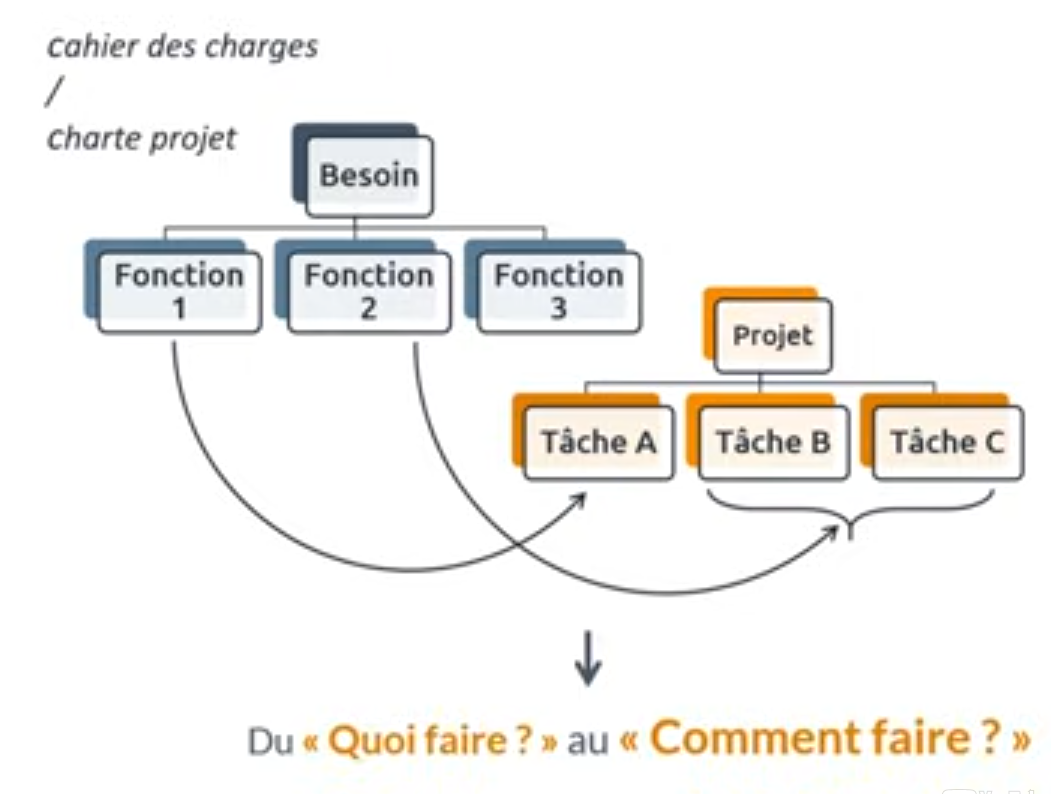
\includegraphics[scale=0.2]{images/lots.png}
	\end{center}
\end{figure}
Cela permet d'obtenir l'organigrame des taches, ce qu'on appelle couramment le \textbf{WBS}(work breakdown structure).\\

Pour le PMI, C'est la décomposition hiérachique du travail que l'équipe de projet doit exécuter pour atteindre les objectifs et produire les livrables.
\begin{figure}[!h]
	\begin{center}
		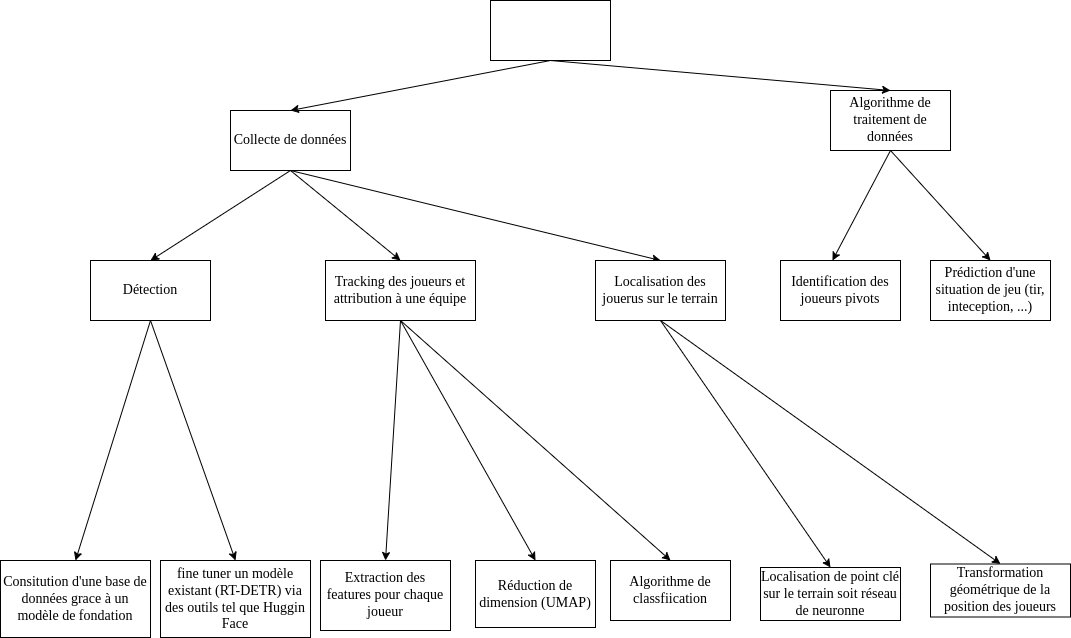
\includegraphics[scale=0.2]{images/wbs.png}
	\end{center}
\end{figure}
\begin{know}
	(source : https://www.wrike.com/fr/project-management-guide/faq/quest-ce-que-le-pmi-en-gestion-de-projet/)\\
	Le PMI, Project Management Institute, est une association professionnelle à but non lucratif qui s'adresse aux chefs de projet et aux chefs de programme. Créée en 1969, elle compte à présent 2,9 millions de professionnels dans le monde. C'est l'organisation qui délivre la qualification PMP (Project Management Professional), un certificat mondialement reconnu qui garantit aux employeurs qu'une personne est formée et qualifiée pour gérer des projets. 
\end{know}
\paragraph*{Les lots de travail / Work packages}
Pour chaque tache de travail, on décompose selon un critère donné. Par exemple le métier qui réalise le travail, la localisation du chantier, l'ordre de succession.
\begin{danger}
	Utiliser un seul critère à la fois.
\end{danger}
\textbf{Chaque lot de travail est un objectif SMART}.\\
Un exemple de WBS à la figure \ref{fig:exemple_wbs}
\begin{figure}[!h]
	\begin{center}
		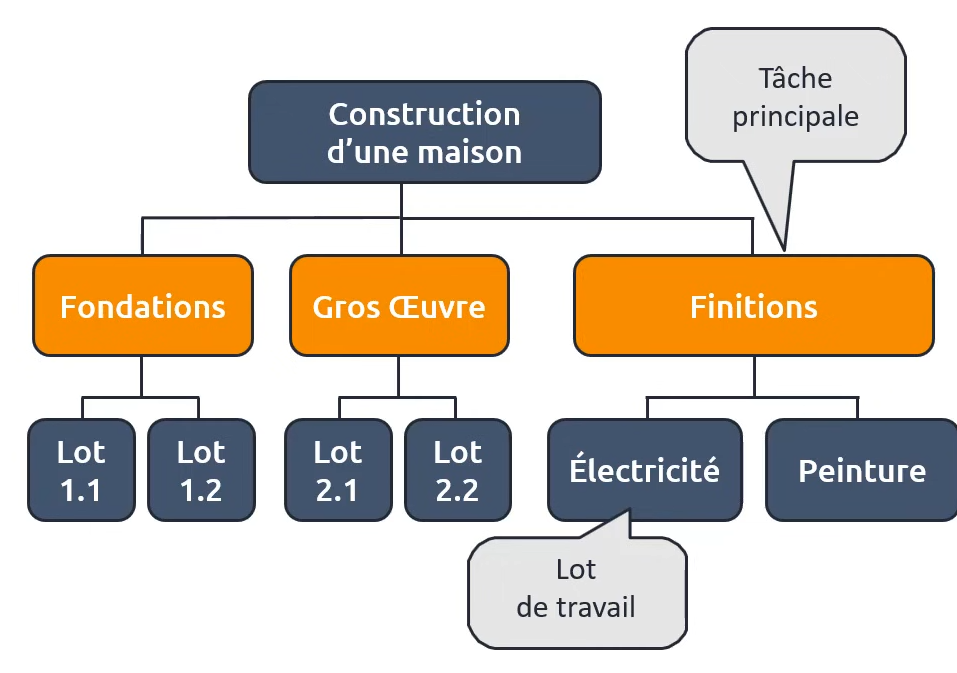
\includegraphics[scale=0.2]{images/exemple_wbs.png}
		\caption{exemple WBS}
		\label{fig:exemple_wbs}
	\end{center}
\end{figure}
\begin{danger}
	\begin{itemize}
		\item Obtenir des lots de travail faciles à maitriser
		\item Si le découpage des taches principales est trop simple, il oublie des éléments importants. Invsersment, s'il est trop détaillé, le projet devient ingérable, car trop complexe.
		\item Enfin chaque lot de travail devra pouvoir etre affecté à un acteur unique.
	\end{itemize}
\end{danger}
\section{Répartition des responsabilités}

\subsection{La matrice RACI}
La \textbf{matrice RACI} est la matrice des responsabilités, elle précise et réparti les roles pour chaque lot de travail, ce qui a pour effet d'éviter les erreurs de communication.

La matrice RACI spécifie quatre types de responsabilités : 
\begin{itemize}
	\item Celui qui \textbf{réalise(R)}
	\item Celui qui a l'\textbf{autorité(A)}
	\item La personne qui \textbf{conseille(C)}
	\item Celel qui est \textbf{informée(I)}
\end{itemize}
\paragraph*{Concevoir une matrice RACI}
\ref{fig:concevoir_matrice_raci}	
\begin{figure}[!h]
	\begin{center}
		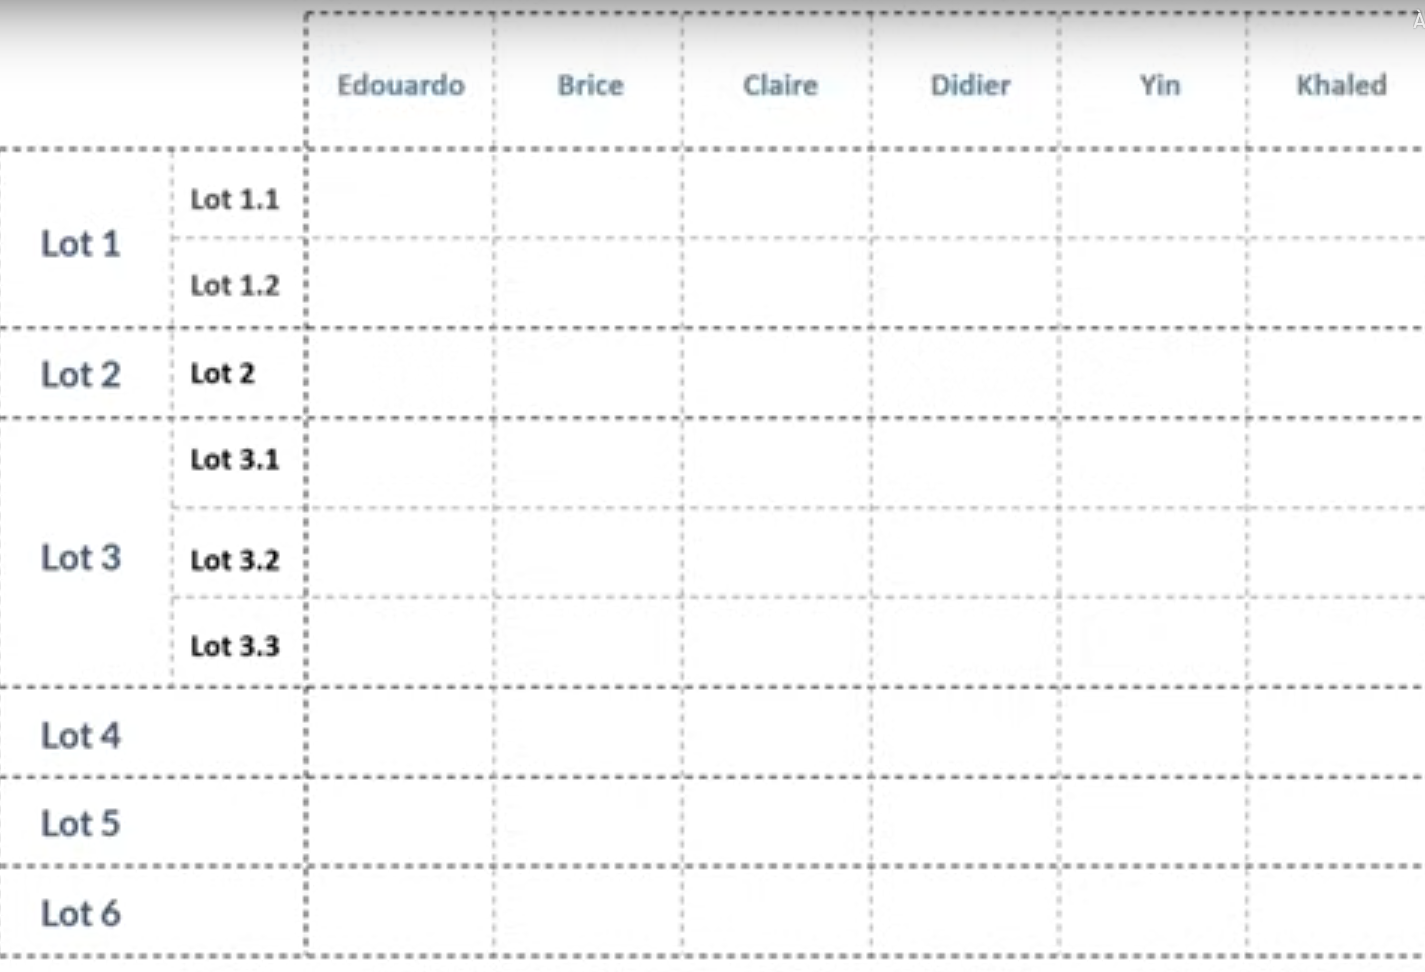
\includegraphics[scale=0.2]{images/modele_matirce_raci.png}
		\caption{Concevoir une matrice RACI}
		\label{fig:concevoir_matrice_raci}
	\end{center}
\end{figure}
\paragraph*{Les responsabilités}
Les 4 types de responsabilités :
\begin{itemize}
	\item Les R sont les membres opérationnels, les réalisateurs du lot de travail. C'est eux qui exécutent la tache.
	\item Le A, c'est l'autorité, celui qui doit rendre des comptes. Le A s'organise comme il veut avec les autres intervenants, mais si le travail n'est pas fait, c'est lui qui assume.
	\item Les C sont généralement ceux qui sont consultés avant la réalisation de certaines taches : ce sont des experts qui apportent les conseils pour préaprer et réussir ce lot de travail.
	\item I, ce sont ceux qui doivent etre tenus informés parcequ'ils sont concernées. Mais ils n'exercent pas un role direct : on avance sans attendre de retour de leur part.
\end{itemize}
\begin{figure}[!h]
	\begin{center}
		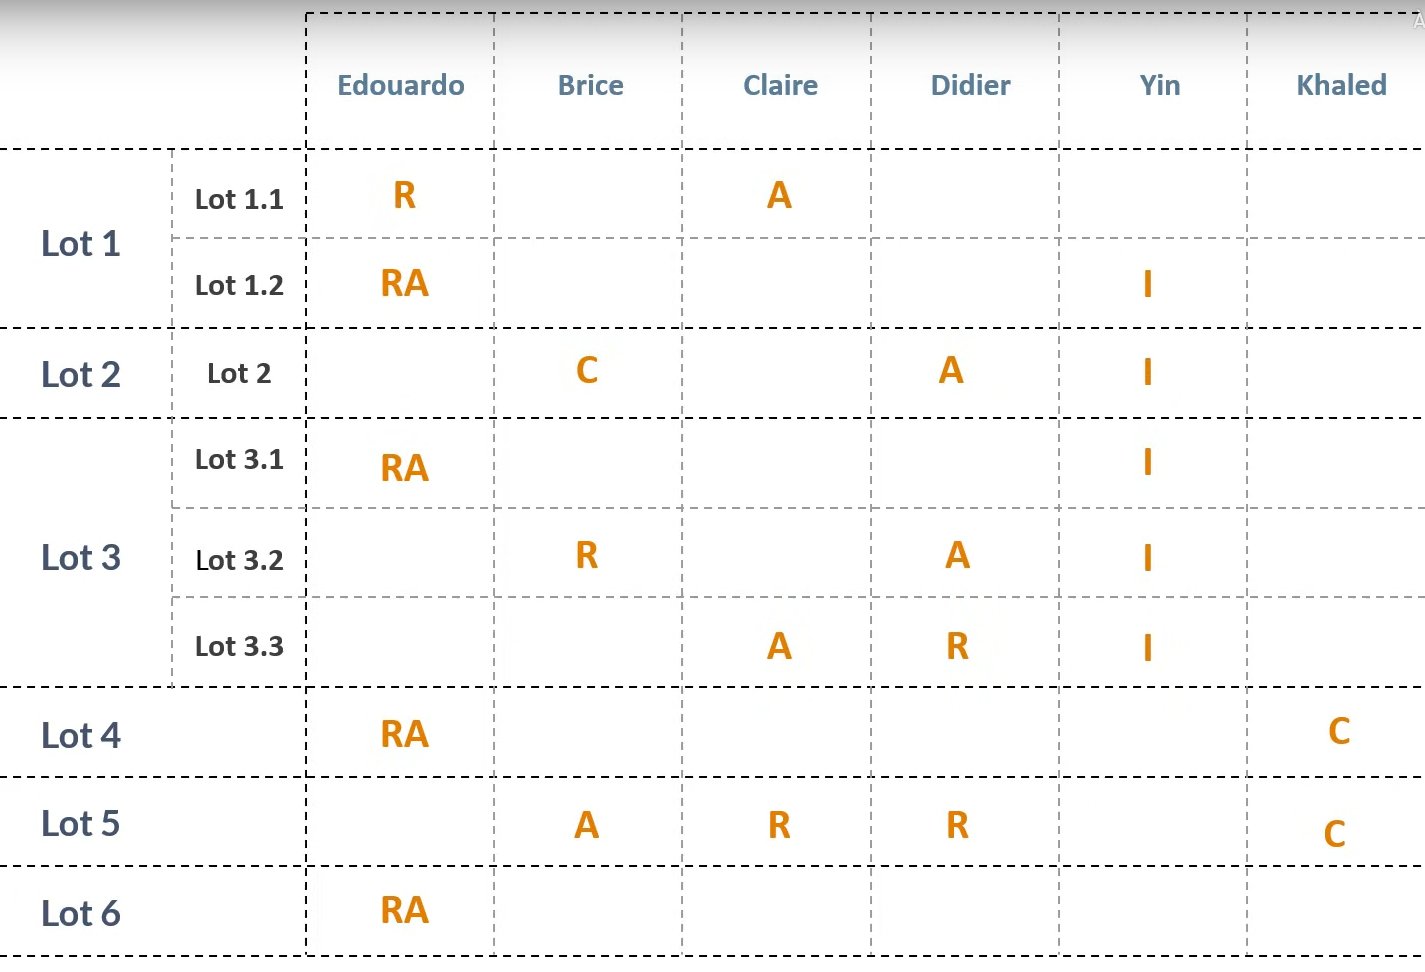
\includegraphics[scale=0.2]{images/exemple_matrice_raci.png}
		\caption{exemple d'une matrice RACI}
	\end{center}
\end{figure}
\textbf{Peut on cumuler des roles?}\\
\begin{danger}
	Pour chaque action il ne doit y avoir qu'un et un seul A, et au moins un R.\\
	Il faut toujours un responsable unique et précis. Il peut néanmoins déléguer certains taches mais il ne doit y avoir qu'une et une seule personne qui a l'autorité finale. Au moins un R parcequ'on peut avoir plusieurs personnes qui réalisent la tache sans poser problème.
	
	\textbf{Pour les taches simples, un seul acteur assume à la fois A et R}.
\end{danger}
La matrice RACI a de nombreuses variantes : P.A.R.i.S, RASCI, RACI-vs, CAIRO, RAPID. Mais RACI est la version la plus souvent utilisée dans le PMI et le sigle RACI marche aussi en anglais (Responsable, Accountable, Consulted, Informed).
\begin{danger}
	\begin{itemize}
	\item Préciser toujours la signification du sigle à coté de notre tableau!
	\item Allez au plus simple : une seule autorité
	\item Pas trop de R
	\item Ne pas multiplier les C : plus on consulte, plus on ralenti. Il faut consulter directement les experts les plus efficaces.
	\item Gardez tous les acteurs du projet informés sinon on vous reprochera de mal communiquer.
\end{itemize}
\end{danger}
\paragraph*{Limites de la matrice RACI}
La principale, c'est quelle ne clarifie pas la répartition des actions précises. Autrement dit, elle ne suffit pas, il faut la combiner avec le PDCA.

\begin{danger}
Activité : Créez le WBS et la matrice RACI de votre projet !\\
Lien drive : https://docs.google.com/presentation/d/1qgz5mPLzQJj33rGQ4Iffm36zu62yk7Q1vNtGxL4J9As/edit\#slide=id.g30f4a5e4f6\_0\_98\\
Lien pptx : https://drive.google.com/file/d/1lhFmlW0Q100cVBPJ4a71Y2\_NzGtW8T2w/view
\end{danger}
\begin{figure}[!h]
	\begin{center}
		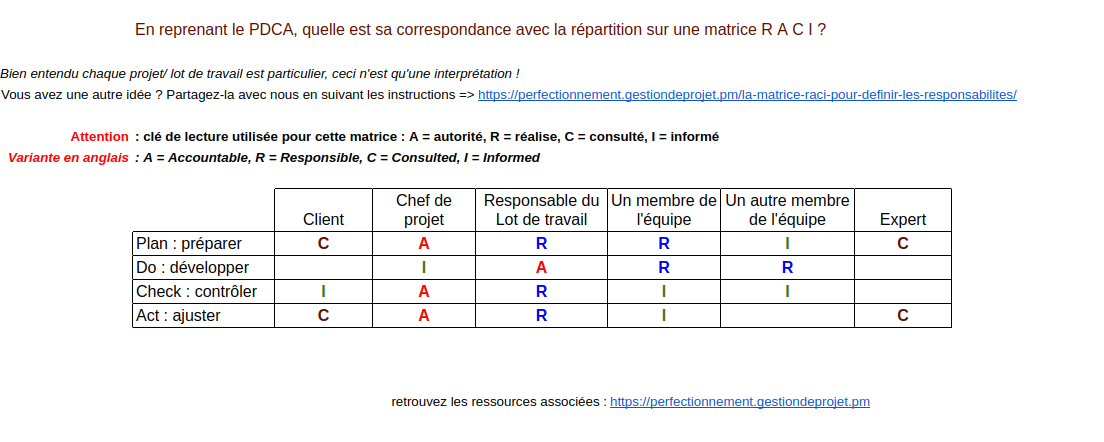
\includegraphics[scale=0.6]{images/correpondance_pdca_raci.png}
		\caption{Matrice correpondance PDCA avec RACI : https://docs.google.com/spreadsheets/d/1kKR2M73T5\_v2OcCzTcH6CKf0niMiJnM9C2VdAqlvanY/pubhtml}
	\end{center}
\end{figure}
\section{Plannification}
\paragraph*{Séquencement des work packages : diagramme de PERT}
C'est donner pour chaque lot de travail, son ordre de succession.
\begin{figure}[!h]
	\begin{center}
		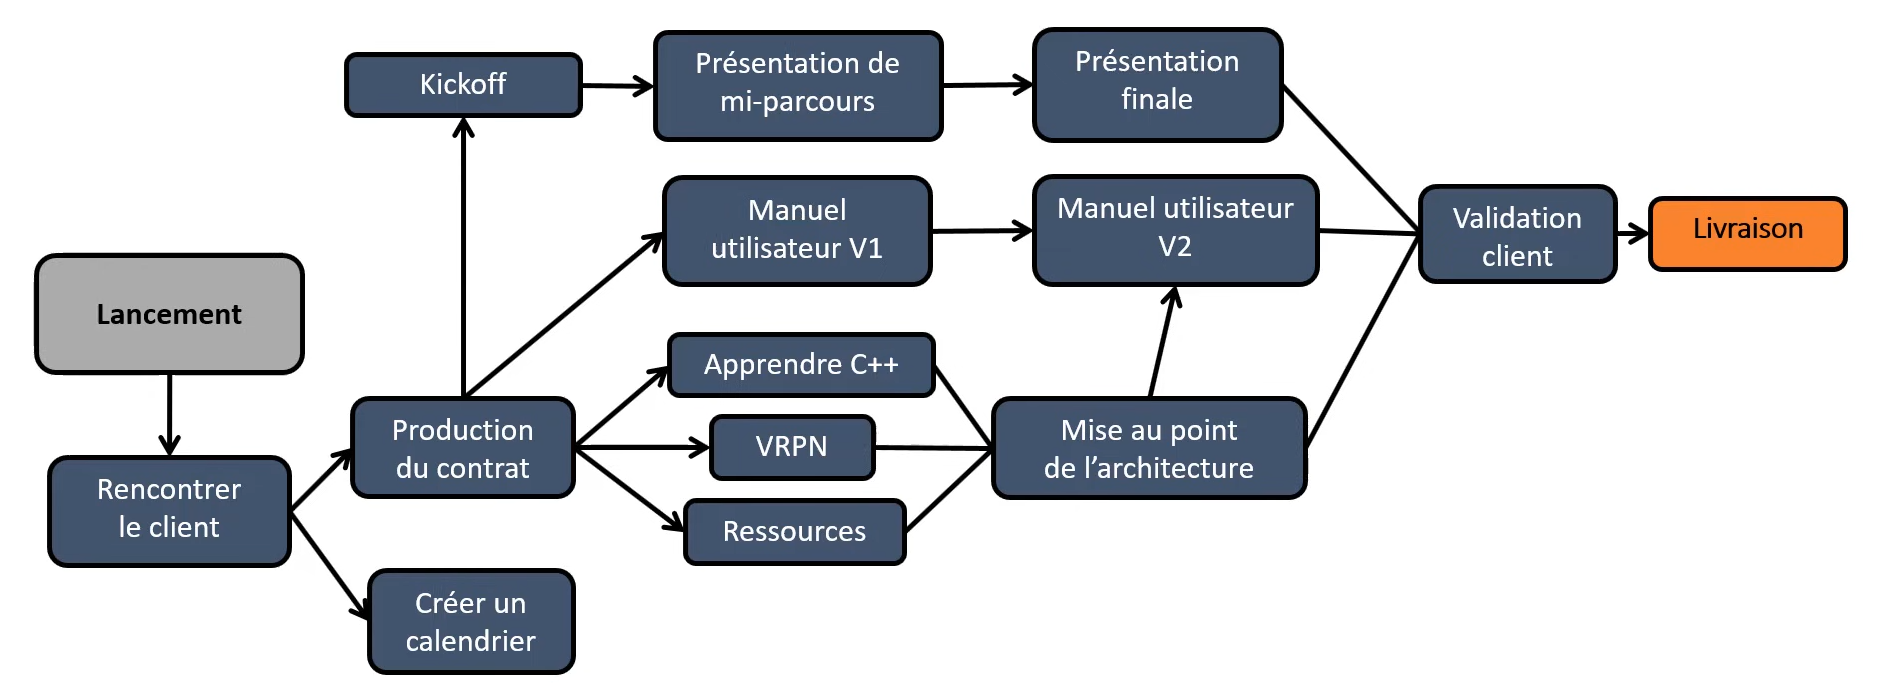
\includegraphics[scale=0.2]{images/exemple_sequencement_lots.png}
		\caption{Exemple de séquencement des lots de travial}
	\end{center}
\end{figure}
\paragraph*{Diagramme de Gantt prévisionnel}
\begin{itemize}
	\item Les lots de travail sont représentées par des barres
	\item Les jalons sont représentés par des losanges
	\item Les flêches indiquent les liens entre les tâches
	\item Le chemin critique qui détermine la date de fin du projet
\end{itemize}
\begin{figure}[!h]
	\begin{center}
		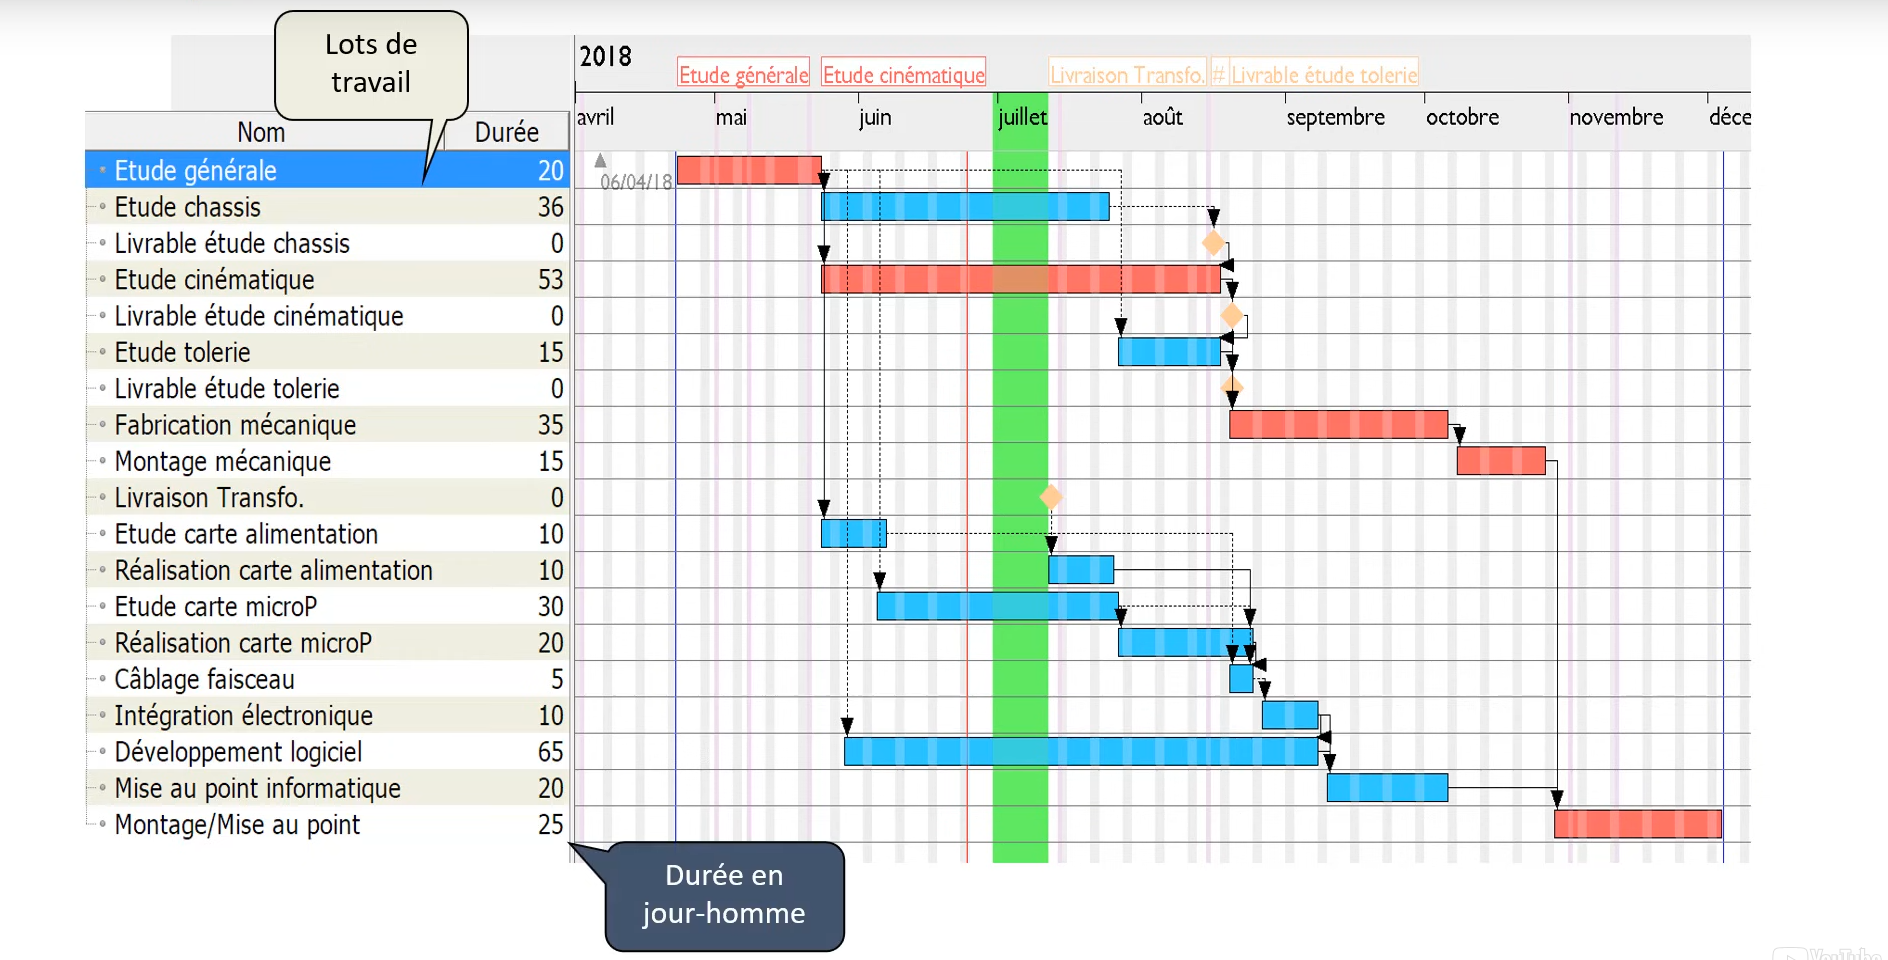
\includegraphics[scale=0.2]{images/exemple_diagramme_gantt.png}
		\caption{Exemple de diagramme de Gantt prévisionnel}
	\end{center}
\end{figure}
\begin{figure}[!h]
	\begin{center}
		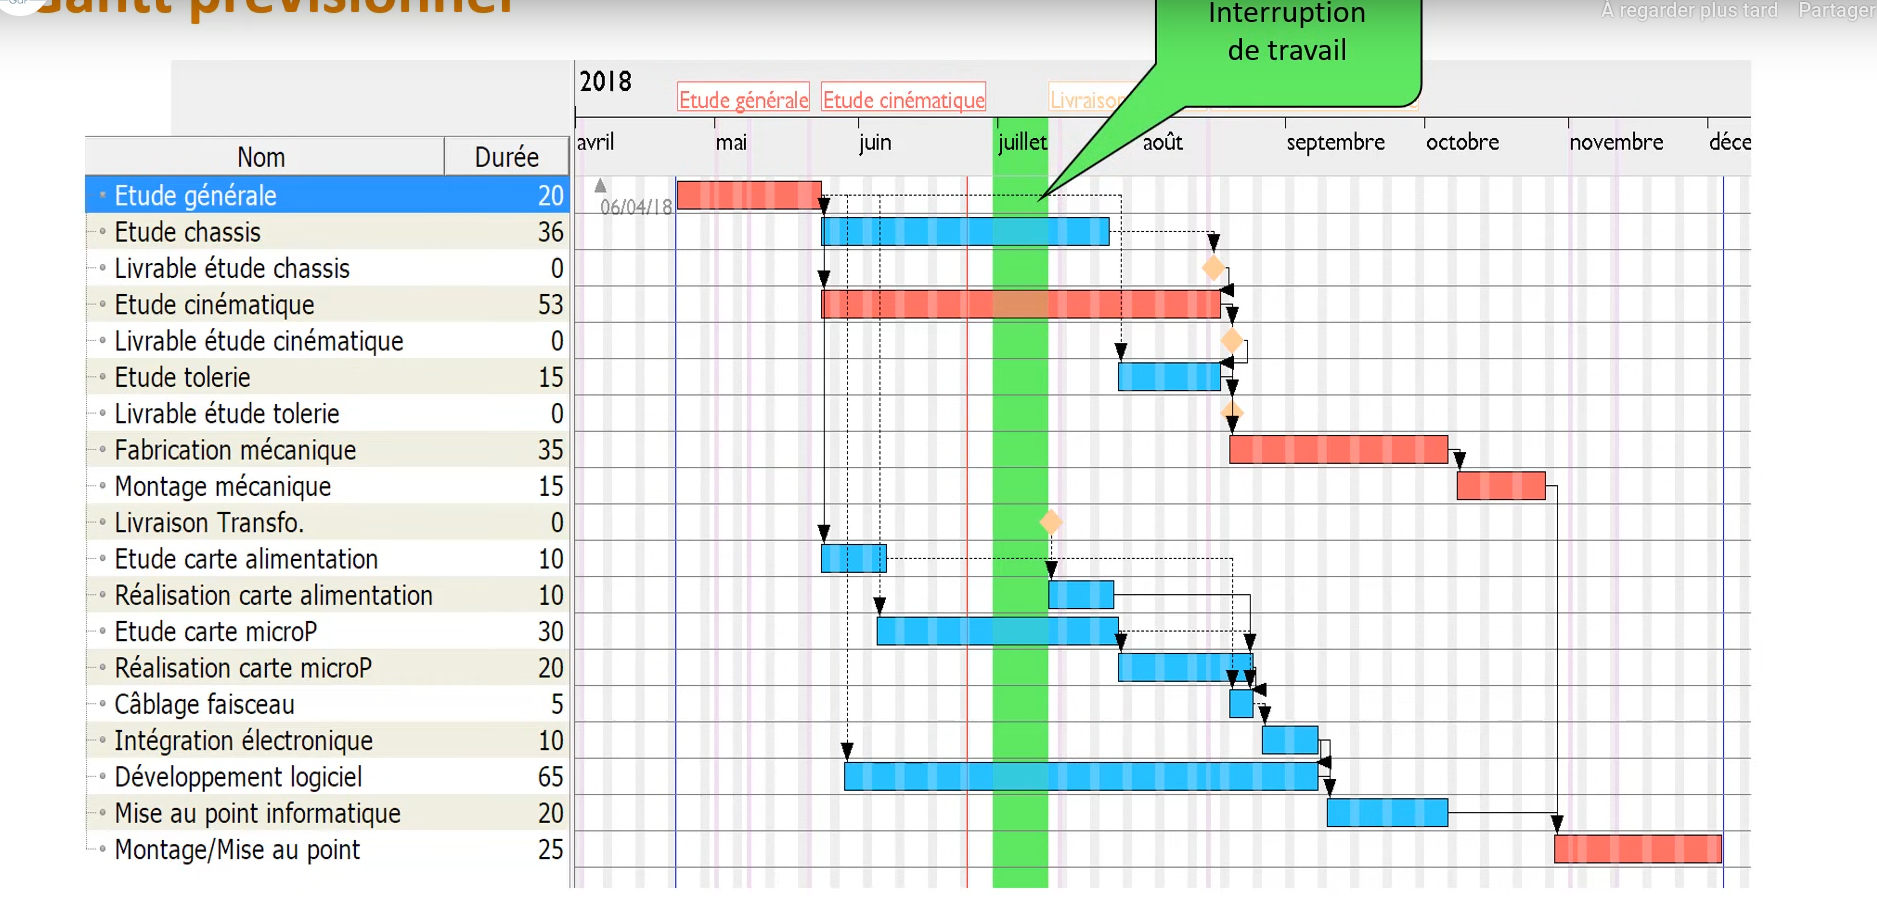
\includegraphics[scale=0.2]{images/exemple_diagramme_gantt1.png}
		\caption{Exemple de diagramme de Gantt prévisionnel (illustration période interruption)}
	\end{center}
\end{figure}
\begin{figure}[!h]
	\begin{center}
		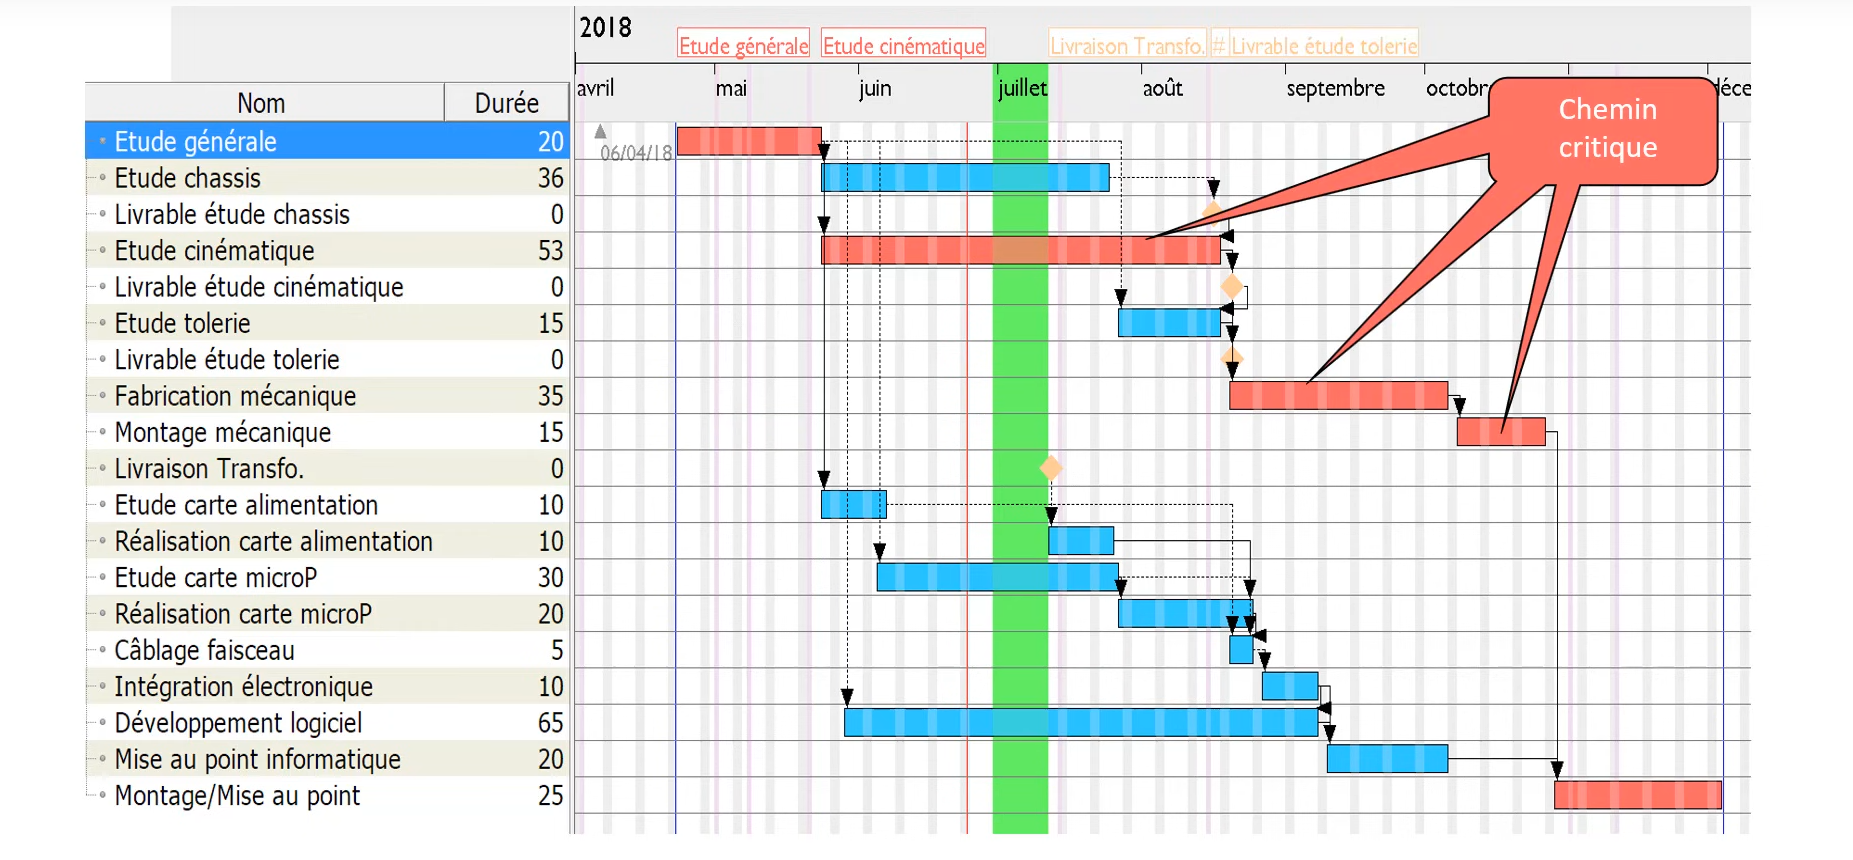
\includegraphics[scale=0.2]{images/exemple_diagramme_gantt2.png}
		\caption{Exemple de diagramme de Gantt prévisionnel (illustration chemin critique)}
	\end{center}
\end{figure}
\paragraph*{Diagramme de Gantt en mode pilotage}
\begin{figure}[!h]
	\begin{center}
		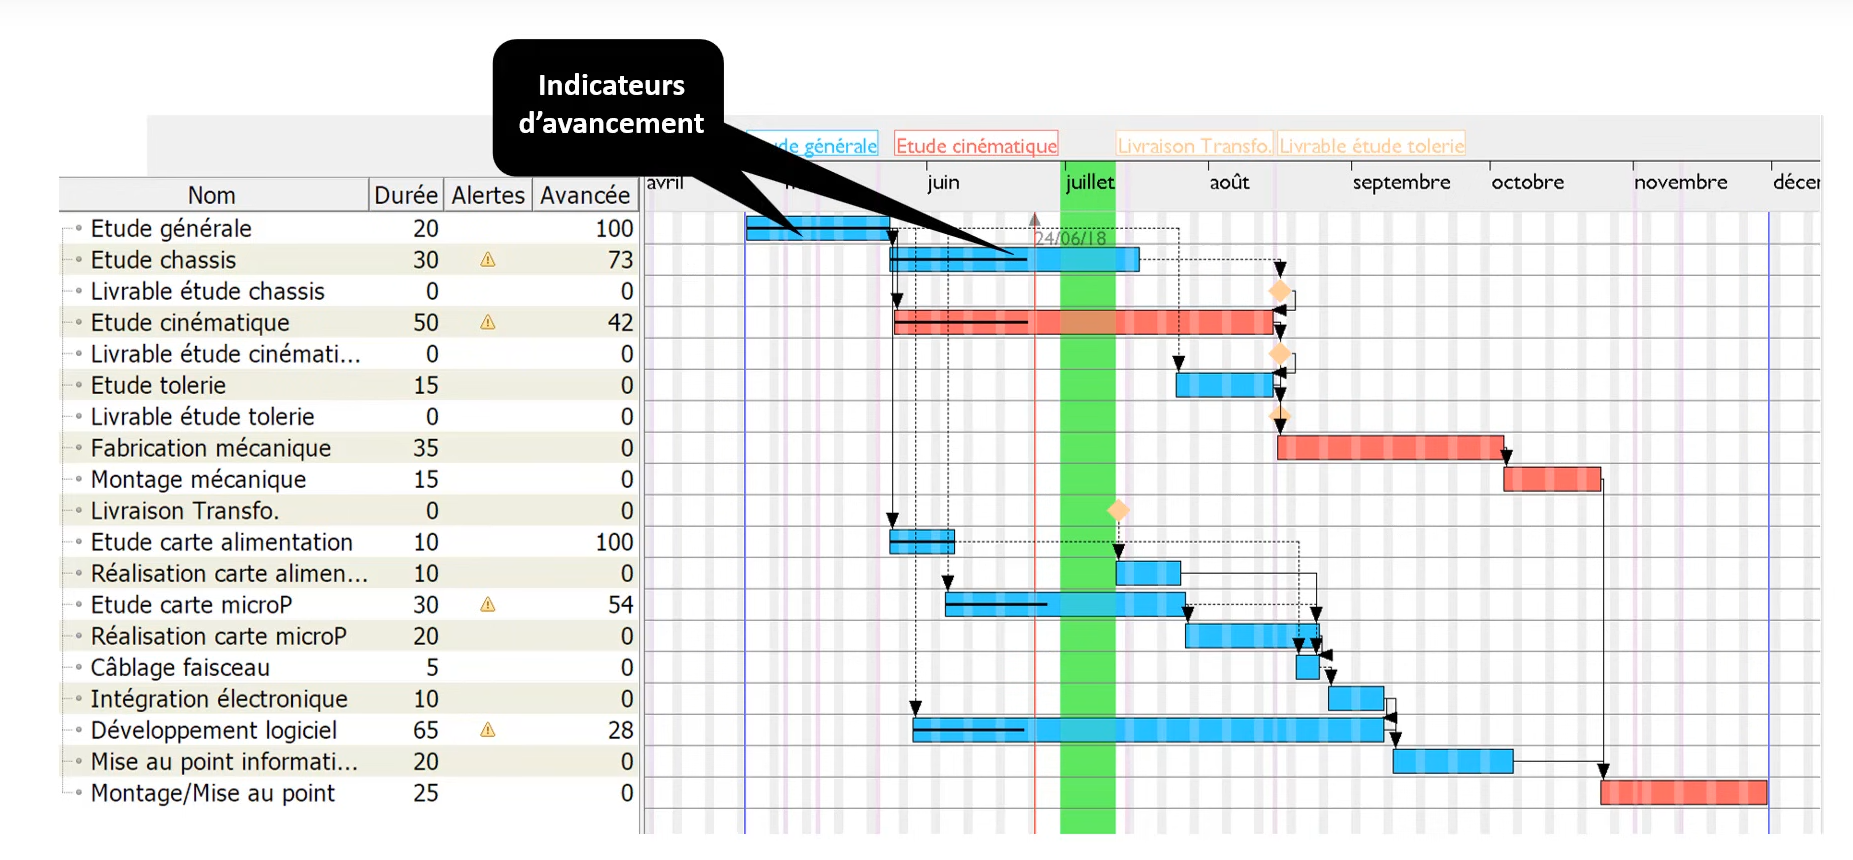
\includegraphics[scale=0.2]{images/diagramme_gantt_pilotage1.png}
		\caption{Exemple de diagramme de Gantt en mode pilotage (illustration indicateurs d'avancement)}
	\end{center}
\end{figure}
\begin{figure}[!h]
	\begin{center}
		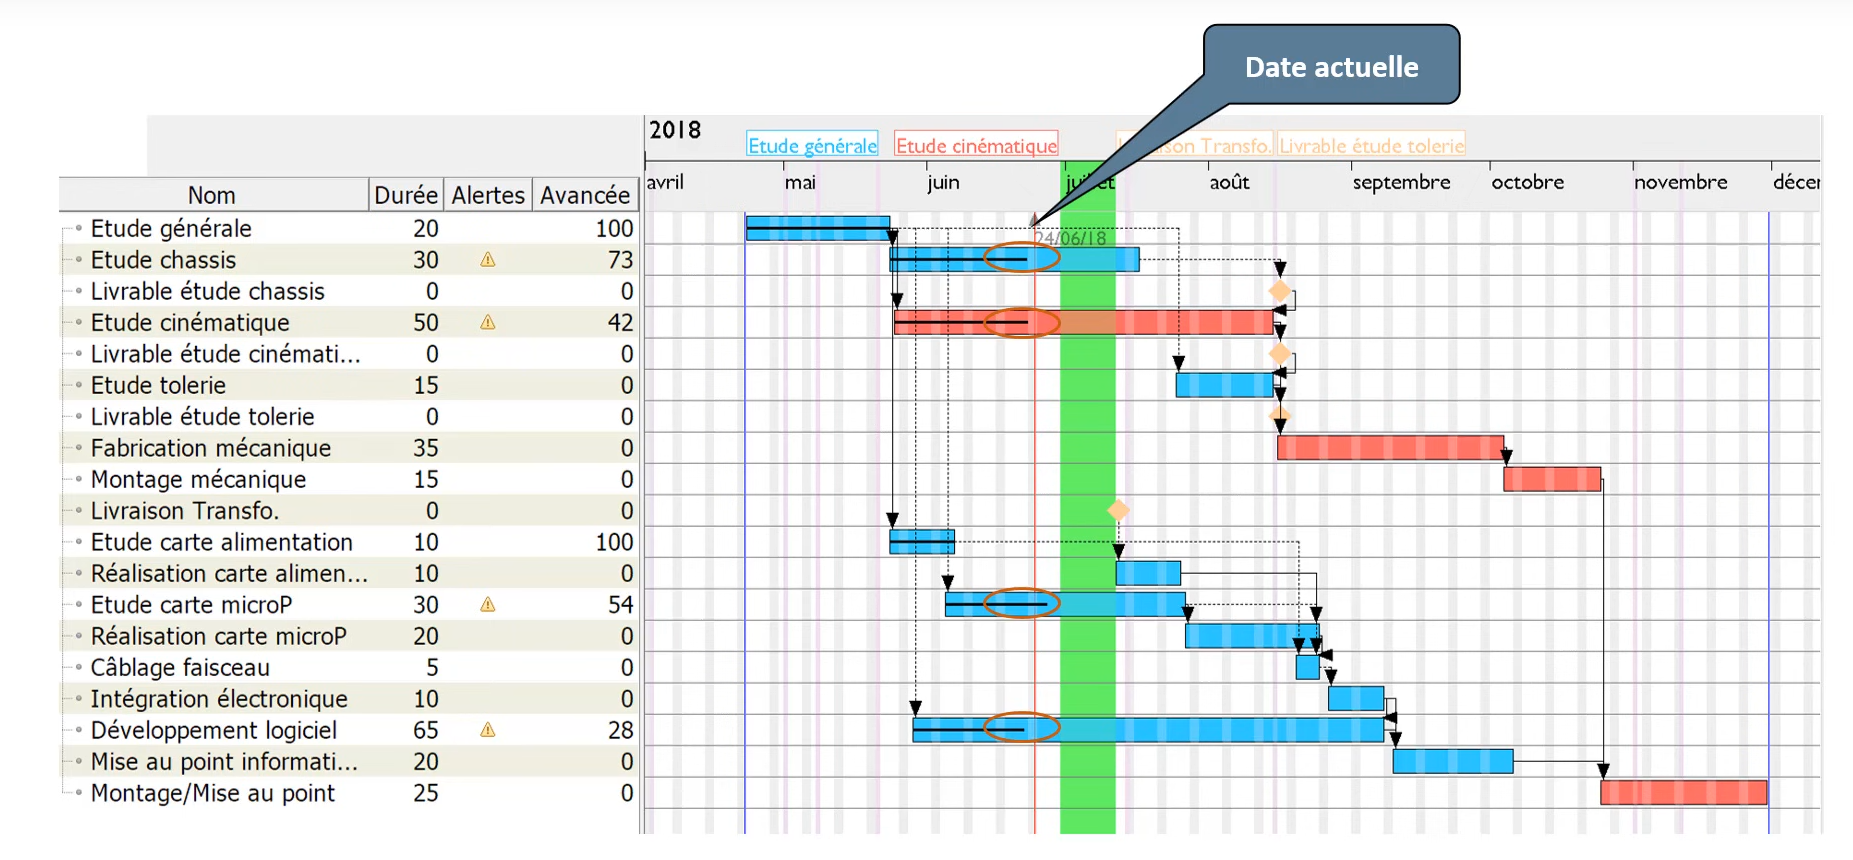
\includegraphics[scale=0.2]{images/diagramme_gantt_pilotage.png}
		\caption{Exemple de diagramme de Gantt en mode pilotage (illustration (se servir de la date actuelle pour voir si on est en retard))}
	\end{center}
\end{figure}